\documentclass{article}
\usepackage[final,main]{neurips_2025}  % NEURIPS style (neurips_2025.sty is in paper_draft/); main = main track

\usepackage[utf8]{inputenc}
\usepackage[T1]{fontenc}
\usepackage[hidelinks]{hyperref}  % REQUIRED: clickable links
\usepackage{booktabs}  % REQUIRED: professional tables
\usepackage{graphicx}
\usepackage{amsmath,amssymb}
\usepackage{natbib}
\usepackage{subcaption}
\usepackage{xspace}
\usepackage{enumitem}
\usepackage{multirow}
\usepackage{algorithm}
\usepackage[noend]{algpseudocode}  % provides \algorithmicindent referenced in commands/general.tex

% Import command files
\input{commands/math}
\input{commands/general}
\input{commands/macros}

% Use this bibliography style:
\bibliographystyle{plainnat}

\title{The Novelty Mirage: A Controlled Ablation of Six Grounding\\ Mechanisms for LLM Scientific Idea Generation}

\author{Chenhao Tan and NeuriCo}

\begin{document}
\maketitle

\begin{abstract}
Large language models (LLMs) now generate research ideas that human experts judge more novel than their own, yet the field distrusts these ideas because ``novelty'' is poorly defined. A natural fix is to \emph{ground} the abstract notion of novelty in a concrete reasoning process. Six such mechanisms have been proposed in isolation---deduction, induction, proposal writing, outcome imagination, small experiments, and literature comparison---but no study compares them under one controlled protocol. We run the first head-to-head ablation: one fixed backbone (\gptfourone), the canonical 7 NLP ideation topics, an identical output schema across all conditions, and 5 replicates per cell, for 245 ideas. We evaluate with three independent lenses: an objective embedding metric (distance to 1{,}050 real prior-work abstracts), a 2-judge off-family LLM rubric, and position-controlled pairwise comparisons. Grounding does \emph{not} uniformly improve quality; instead each mechanism steers the novelty--feasibility trade-off in a specific way. Crucially, the apparent novelty gains exist almost entirely in the LLM judge's eye: they vanish under the objective metric, with which judge novelty is \emph{completely uncorrelated} (Spearman $\rho = 0.01$). Literature comparison wins 79\% of head-to-head comparisons and is the only mechanism that raises idea-set diversity, while ``small experiment'' grounding actively hurts novelty by pulling ideas toward already-published methods. Our results give a controlled, quantitative confirmation of the ``novelty mirage'' and argue that single-number LLM-judged novelty should never be reported alone.

\end{abstract}

\section{Introduction}
\label{sec:intro}

LLM scientific ideation has crossed a surprising threshold. In a controlled study with more than 100 NLP researchers, ideas produced by an LLM agent were judged \emph{more novel} than those written by expert humans~\citep{si2024can}. Yet the field still distrusts machine-generated ideas, and for a concrete reason: ``novelty'' is ill-defined. Unguided LLMs swing between incremental rephrasings of known work and implausible over-reaches, and the very judgments that crown them as novel come from other LLMs whose reliability is in question.

A natural and inexpensive fix is to \emph{ground} the abstract notion of novelty in a concrete reasoning process before an idea is committed. Rather than asking a model to ``be novel,'' one can ask it to flip a stated assumption, induce a hypothesis from observations, draft a full proposal, imagine the most surprising plausible outcome, design a falsification test, or explicitly contrast its idea against retrieved prior work. Each of these is a cheap prompting protocol, not a new model, so if any reliably moves ideas toward the novel-and-plausible sweet spot it would directly improve automated discovery pipelines at almost no cost.

\para{The gap.} Every strong prior system champions \emph{one} grounding mechanism, evaluated on \emph{its own} dataset and metric: literature comparison in SciMON, Chain-of-Ideas, and Nova~\citep{wang2023scimon,li2024chain,nova2024}; induction in MOOSE and causal-graph hypothesis generation~\citep{yang2023moose,causalgraph2024}; deduction in HypoGen's Bit$\rightarrow$Flip$\rightarrow$Spark schema~\citep{hypogen2025}; proposal writing in the Si agent and VirSci~\citep{si2024can,virsci2024}; outcome imagination in AutoDiscovery's Bayesian surprise~\citep{autodiscovery2025}; and critic/small-experiment feedback in Deep-Ideation~\citep{deepideation2025}. \emph{No paper compares these six mechanisms head-to-head under one controlled protocol}---same backbone, same seed topics, same metrics, same output format. Two evaluation-skeptic papers~\citep{glitters2025,rqbench2026} add that the \emph{evaluation} itself must be grounded, not left to a single LLM's opinion. Whether grounding helps is therefore essentially untested as a controlled ablation, and how to measure ``help'' is itself contested.

\para{Our approach.} We run the first controlled head-to-head ablation of all six grounding mechanisms plus an unguided control. We hold the backbone (\gptfourone), the seed topics (the 7 canonical NLP topics of \citet{si2024can}), and the output schema fixed, varying \emph{only} the reasoning scaffold that precedes the idea; this isolates grounding from the length and format confounds that complicate prior comparisons. We generate 5 replicates per cell, for 245 ideas, and evaluate them through three independent lenses: (i)~an \emph{objective} literature-grounded novelty metric (\lgn), the embedding distance from each idea to the nearest of 1{,}050 real prior-work abstracts retrieved from Semantic Scholar; (ii)~a 2-judge rubric using \claudesonnet and \geminiflash, both deliberately off-family from the backbone to limit self-preference; and (iii)~position-controlled pairwise comparisons against the control.

\para{What we find.} The three lenses disagree, and the disagreement is the headline. Grounding does not uniformly improve quality---it \emph{steers} the novelty--feasibility trade-off. Deduction and literature comparison raise judged novelty (Cohen's $d = 0.81$ and $0.57$), and literature comparison wins 79\% of head-to-head comparisons against the control while being the only mechanism that improves idea-set diversity. But \emph{no} mechanism increases objective distance from prior work; the only significant effect there is proposal writing making ideas \emph{more} conventional. Most strikingly, LLM-judged novelty and objective novelty are uncorrelated at the item level (Spearman $\rho = 0.01$, $p = 0.85$), even though the two judges agree with each other ($\rho = 0.41$). The novelty gains are real in the judge's eye and a mirage under a literature-anchored measure---a clean, controlled reproduction of the ``novelty mirage''~\citep{rqbench2026}.

\para{Contributions.}
\begin{itemize}[leftmargin=*,itemsep=0pt,topsep=0pt]
    \item We conduct the first controlled head-to-head ablation of six grounding mechanisms for LLM idea generation, isolating the reasoning scaffold from backbone, topic, and output-format confounds across 245 ideas.
    \item We complement the standard LLM-judge rubric with an objective, judge-independent literature-grounded novelty metric and a convergent-validity test, and show that judged novelty is uncorrelated with objective novelty---a direct, quantitative confirmation of the novelty mirage.
    \item We characterize each mechanism's effect as a position on the novelty--feasibility axis, and distill practical guidance: use literature comparison for judged novelty and diversity, induction or proposal writing for feasibility, and never report single-LLM-judge novelty alone.
\end{itemize}

The rest of the paper reviews related work (\secref{sec:related}), details our protocol and metrics (\secref{sec:method}), presents results across the three lenses (\secref{sec:results}), and discusses implications and limitations (\secref{sec:discussion}).

\section{Related Work}
\label{sec:related}

\para{LLM scientific ideation and its weaknesses.} The pivotal empirical result is \citet{si2024can}, who ran a blind study with 49 expert idea writers and 79 reviewers across 7 NLP topics. Their LLM agent---RAG over retrieved papers, over-generation of thousands of seeds, deduplication, and pairwise tournament ranking---produced ideas judged \emph{more novel} than expert humans, but slightly less feasible. The study also exposed two systemic weaknesses that frame much of the follow-up work: \emph{diversity collapse} (thousands of generated seeds yield only a few hundred unique ideas) and \emph{unreliable self-evaluation} (the LLM ranker barely exceeded chance consistency). We reuse their 7 topics and 1--10 rubric so our numbers are comparable, and we directly test whether grounding mitigates diversity collapse.

\para{Grounding via literature comparison.} SciMON~\citep{wang2023scimon} retrieves ``inspirations,'' generates, then iteratively compares each candidate to prior work and revises until it is novel enough. Chain-of-Ideas~\citep{li2024chain} organizes literature into a progression chain and ships a pairwise ``Idea Arena'' evaluation, and Nova~\citep{nova2024} uses planned iterative retrieval to produce more unique top-rated ideas. These systems ground novelty against \emph{retrieved prior work}. Our \litcomp condition implements exactly this retrieve-and-differentiate loop, and our objective \lgn metric is the same idea applied to \emph{evaluation}: distance to retrieved prior work rather than an LLM's opinion.

\para{Grounding via induction and deduction.} MOOSE~\citep{yang2023moose} performs hypothetical induction from a raw corpus to novel social-science hypotheses, refined by feedback. \citet{causalgraph2024} build a causal knowledge graph from tens of thousands of psychology articles and show that an LLM grounded in this inductive structure beats an LLM-only baseline on novelty. On the deductive side, HypoGen~\citep{hypogen2025} introduces the Bit$\rightarrow$Flip$\rightarrow$Spark schema---state the prevailing assumption, invert it, derive the idea---which we adopt verbatim as our \deduction scaffold; HypoSpace~\citep{hypospace2025} evaluates LLMs as set-valued hypothesis generators. Unlike these works, which each validate a single mechanism on a bespoke benchmark, we place induction and deduction on the same footing as four other mechanisms.

\para{Grounding via proposals, outcomes, and experiments.} \citet{dynamiccontrol2024} train SFT+RL reward models for novelty, feasibility, and effectiveness, defining the rubric conventions we follow. VirSci~\citep{virsci2024} uses multi-agent teams to generate, evaluate, and refine full proposals. AutoDiscovery~\citep{autodiscovery2025} drives open-ended discovery by Bayesian surprise---the epistemic shift after running experiments---which motivates our \outcome scaffold. Deep-Ideation~\citep{deepideation2025} evolves ideas over a concept network using a critic trained on real reviewer feedback, which we operationalize as our \smallexp scaffold (design a falsification test, predict its result, self-critique, revise). Because generic ideas cannot be cheaply executed in-loop, we follow the predict-and-critique operationalization used by MOOSE and Deep-Ideation.

\para{Grounding the evaluation.} Two recent papers warn that the metric, not just the generator, must be grounded. \emph{All That Glitters Is Not Novel}~\citep{glitters2025} finds that a quarter of ``novel'' AI research documents are smartly borrowed and bypass detectors, recommending that novelty be measured as distance to retrieved prior work. \emph{On the Limits of LLM-as-Judge}~\citep{rqbench2026} documents a \emph{novelty mirage}: LLM judges rate model-generated questions as highly novel while human experts prefer the real references. These cautions motivate our three-lens evaluation and the convergent-validity test that is, to our knowledge, the first controlled measurement of the mirage on a single fixed idea set. Surveys of the area~\citep{survey2025a,survey2025b} report a directional ranking (graph-grounded $3.83 >$ Chain-of-Ideas $3.21 >$ vanilla $2.44$) suggesting grounding helps novelty; our objective metric and overall-quality scores caution that this ranking may itself be judge-inflated.

\section{Methodology}
\label{sec:method}

\para{Research question.} Do LLMs generate higher-quality scientific ideas---more novel \emph{and} still feasible---when the abstract notion of novelty is grounded through one of six mechanisms, versus unguided generation, holding the backbone model, seed topic, and output format fixed? We decompose this into five hypotheses. \textbf{H1} (objective novelty): grounded conditions produce ideas with greater embedding distance to prior work. \textbf{H2} (judged quality): grounded conditions score higher on the rubric and win $>50\%$ of pairwise comparisons. \textbf{H3} (no feasibility collapse): grounding does not significantly reduce feasibility. \textbf{H4} (diversity): grounding increases set-level diversity. \textbf{H5} (evaluation): judge novelty correlates with the objective metric; if not, this supports the novelty-mirage caution.

\subsection{Design}

We use a fully crossed $7~(\text{condition}) \times 7~(\text{topic})$ design with 5 replicates per cell, for $7 \times 7 \times 5 = 245$ ideas. The independent variable is the grounding condition; topic is a blocking variable; the backbone, sampling parameters, seed text, and output schema are fixed.

\para{Critical control.} Every condition emits the \emph{identical} idea JSON schema (\texttt{title}, \texttt{problem}, \texttt{motivation}, \texttt{method}, \texttt{experiment\_plan}); only the reasoning \emph{scaffold} preceding the idea differs. This isolates grounding from the output-format and length confounds noted by \citet{si2024can}, whose AI ideas were systematically longer than human ones. Mean idea length is balanced across conditions (199--236 words), and we log idea length and re-run every test with length as a covariate. All effects are robust to this covariate, with $p$-values essentially unchanged (\secref{sec:results}), so our results are not a length artifact.

\para{Conditions.} The seven scaffolds, all ending in the same schema, are:
\begin{itemize}[leftmargin=*,itemsep=1pt,topsep=2pt]
    \item \unguided (control): ``propose a novel idea on \textsc{topic},'' single shot.
    \item \deduction: HypoGen Bit$\rightarrow$Flip$\rightarrow$Spark---state the prevailing assumption, invert it, derive the idea~\citep{hypogen2025}.
    \item \induction: present concrete observations on the topic, induce a general hypothesis, then the idea~\citep{yang2023moose}.
    \item \proposal: draft a full mini-proposal including expected results, then distill the idea~\citep{si2024can}.
    \item \outcome: imagine the best plausible empirical outcome and the belief it would shift, then back out the idea~\citep{autodiscovery2025}.
    \item \litcomp: retrieve 8 real prior papers, explicitly contrast, and revise the idea until distinct~\citep{wang2023scimon}.
    \item \smallexp: design a falsification test, predict its result, self-critique, and refine~\citep{deepideation2025}.
\end{itemize}

\para{Topics.} We use the 7 NLP topics of \citet{si2024can}---Bias, Coding, Safety, Multilingual, Factuality, Math, and Uncertainty---phrased as identical standardized seeds across all conditions.

\subsection{Models and corpus}

\para{Backbone.} The generator is \gptfourone (temperature 0.8, top-$p$ 1.0, max 1600 tokens) with a per-cell deterministic seed, fixed across all conditions.

\para{Judges.} We use two judges deliberately chosen \emph{off-family} from the backbone to limit self-preference: \claudesonnet and \geminiflash, both at temperature 0. Each scores the \citet{si2024can} 1--10 rubric (novelty, feasibility, effectiveness, overall) and renders pairwise preferences.

\para{Objective metric.} Literature-Grounded Novelty (\lgn) is $1 - \max$ cosine similarity of an idea to the nearest prior-work abstract, using 150 recent abstracts per topic (1{,}050 total) retrieved from the Semantic Scholar Graph API and embedded with \mpnet. Higher \lgn means more distant from real prior work. No LLM opinion is involved, so \lgn is judge-independent by construction.

\subsection{Metrics and statistical analysis}

We report four metric families: (i)~\lgn (objective novelty, primary); (ii)~the 1--10 rubric scores; (iii)~pairwise win-rate of each grounded condition against the unguided control, controlling for position by running both orderings with both judges; and (iv)~set-level diversity, the mean pairwise embedding distance within a (condition $\times$ topic) cell, plus a near-duplicate rate (fraction of pairs with cosine $\geq 0.8$).

For the per-idea metrics we fit a linear mixed-effects model, $\text{metric} \sim C(\text{condition}, \text{ref}=\unguided) + (1\,|\,\text{topic})$, reporting coefficients, 95\% confidence intervals, $p$-values, and Cohen's $d$ versus the control. We correct for multiple comparisons with the Holm procedure across the 6 grounded conditions, at $\alpha = 0.05$. Pairwise win-rates are tested against chance (0.5) with a $t$-test and bootstrap 95\% CI. For judge validation we report the Spearman correlation between the two judges' novelty scores (inter-judge agreement) and between mean judge novelty and \lgn (convergent validity). Seeds are fixed at 42 and every LLM call is cached on disk, so the full pipeline reproduces exactly: a second generation pass produced 245/245 cache hits and zero API calls. Total cost was roughly \$3--4 of API usage and about 25 minutes of runtime, with a single RTX A6000 used only for embeddings.

\section{Results}
\label{sec:results}

We present results through the three lenses in turn---objective novelty (\secref{sec:res_lgn}), the judge rubric and pairwise comparisons (\secref{sec:res_judge}), set-level diversity (\secref{sec:res_div})---and close with the judge-validation test that ties them together (\secref{sec:res_valid}). The headline is that the lenses \emph{disagree}, in a way that is itself the main finding.

\subsection{Objective literature-grounded novelty: no grounding helps}
\label{sec:res_lgn}

\Tabref{tab:lgn} reports \lgn relative to the unguided control. \emph{No grounding mechanism significantly increases objective novelty.} The only Holm-significant effect is in the wrong direction: \proposal makes ideas \emph{more} conventional---closer to existing work---than the control ($d = -0.66$, Holm $p = 0.007$). \induction and \outcome trend the same way ($d = -0.40$ and $-0.34$) but do not survive correction. \deduction and \litcomp, the two conditions that most raise \emph{judged} novelty (\secref{sec:res_judge}), are statistically indistinguishable from the control on \lgn ($d = 0.09$ and $0.01$). H1 is refuted: grounding does not move ideas farther from real prior work, and one mechanism pulls them closer. \Figref{fig:lgn} shows the same picture.

\begin{table}[t]
    \centering
    \caption{Objective literature-grounded novelty (\lgn) by condition, from the mixed-effects model with \unguided as reference. Higher \lgn means more distant from real prior work. Effects are robust to a length covariate (rightmost column). The only Holm-significant effect makes ideas \emph{less} novel. Best (most novel) grounded value in \textbf{bold}; the significant effect is marked \checkmark.}
    \label{tab:lgn}
    \begin{tabular}{@{}lccccc@{}}
        \toprule
        Condition & \lgn mean & Cohen's $d$ & $p$ & Holm $p$ & $p$ (len.\ cov.) \\
        \midrule
        \unguided (control)   & 0.188 & ---    & ---   & ---   & ---   \\
        \midrule
        \deduction            & \textbf{0.190} & $+0.09$ & 0.678 & 1.000 & 0.687 \\
        \litcomp              & 0.188 & $+0.01$ & 0.971 & 1.000 & 0.984 \\
        \smallexp             & 0.181 & $-0.19$ & 0.334 & 1.000 & 0.393 \\
        \outcome              & 0.176 & $-0.34$ & 0.089 & 0.358 & 0.090 \\
        \induction            & 0.174 & $-0.40$ & 0.044 & 0.219 & 0.045 \\
        \proposal             & 0.165 & $-0.66$ & 0.001 & \textbf{0.007}~\checkmark & 0.001 \\
        \bottomrule
    \end{tabular}
\end{table}

\begin{figure}[t]
    \centering
    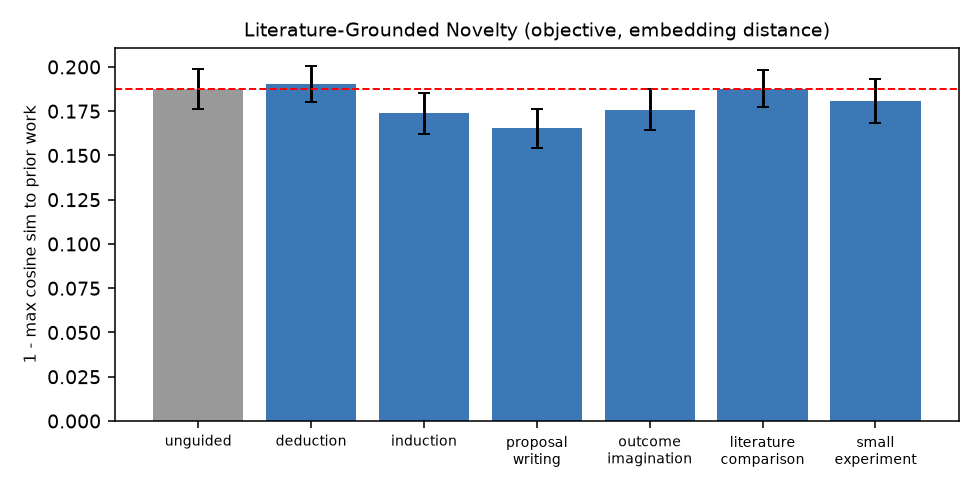
\includegraphics[width=0.62\linewidth]{figures/fig1_lgn.png}
    \caption{Objective literature-grounded novelty (\lgn) by condition, with the unguided control marked. No grounding mechanism rises above the control; \proposal sits significantly below it. Grounding does not increase genuine distance from prior work.}
    \label{fig:lgn}
\end{figure}

\subsection{Judge rubric and pairwise comparisons: a steered trade-off}
\label{sec:res_judge}

The LLM judges tell a very different story (\Tabref{tab:rubric}). On \emph{judged} novelty, \deduction is the clear winner ($5.94$ vs.\ $5.49$, $d = +0.81$, Holm-significant), with \litcomp and \outcome also up ($d = +0.57$ and $+0.59$). But these gains come with a feasibility cost. The conditions split into two clean clusters. \emph{Generative} grounding (\deduction, \litcomp, \outcome) raises judged novelty but lowers feasibility; \emph{validation} grounding (\smallexp, \induction, \proposal) raises feasibility but leaves novelty flat or lower. \smallexp is the extreme case: it has the highest feasibility ($7.84$, $d = +0.77$) but the lowest novelty ($5.17$, $d = -0.64$) and the only Holm-significant drop in \emph{overall} score ($5.11$, $d = -0.91$). No condition beats the control on overall quality. \Figref{fig:rubric} and the trade-off view in \Figref{fig:tradeoff} make the two clusters visible. H2 is only partially supported (judged novelty, for 2--3 mechanisms), and H3's trade-off is confirmed.

\begin{table}[t]
    \centering
    \caption{Judge rubric scores (1--10, mean over both judges) by condition. \checkmark marks a Holm-significant gain and {\footnotesize\textsf{X}} a Holm-significant loss versus the control. Generative grounding (top group) raises novelty but lowers feasibility; validation grounding (bottom group) does the reverse. No condition improves overall quality, and \smallexp significantly worsens it.}
    \label{tab:rubric}
    \begin{tabular}{@{}lccc@{}}
        \toprule
        Condition & Novelty & Feasibility & Overall \\
        \midrule
        \unguided               & 5.49 & 7.20 & 5.44 \\
        \midrule
        \deduction              & \textbf{5.94}~\checkmark {\scriptsize($d{=}{+}0.81$)} & 6.91 & 5.44 \\
        \litcomp                & 5.80 {\scriptsize($d{=}{+}0.57$)} & 6.83 & 5.36 \\
        \outcome                & 5.70 {\scriptsize($d{=}{+}0.59$)} & 6.89 & 5.46 \\
        \midrule
        \induction              & 5.49 & 7.69 {\scriptsize($d{=}{+}0.59$)} & 5.47 \\
        \proposal               & 5.43 & 7.67 {\scriptsize($d{=}{+}0.54$)} & 5.33 \\
        \smallexp               & 5.17 {\scriptsize($d{=}{-}0.64$)} & \textbf{7.84}~\checkmark {\scriptsize($d{=}{+}0.77$)} & 5.11~{\footnotesize\textsf{X}} {\scriptsize($d{=}{-}0.91$)} \\
        \bottomrule
    \end{tabular}
\end{table}

\begin{figure}[t]
    \centering
    \begin{subfigure}[b]{0.48\textwidth}
        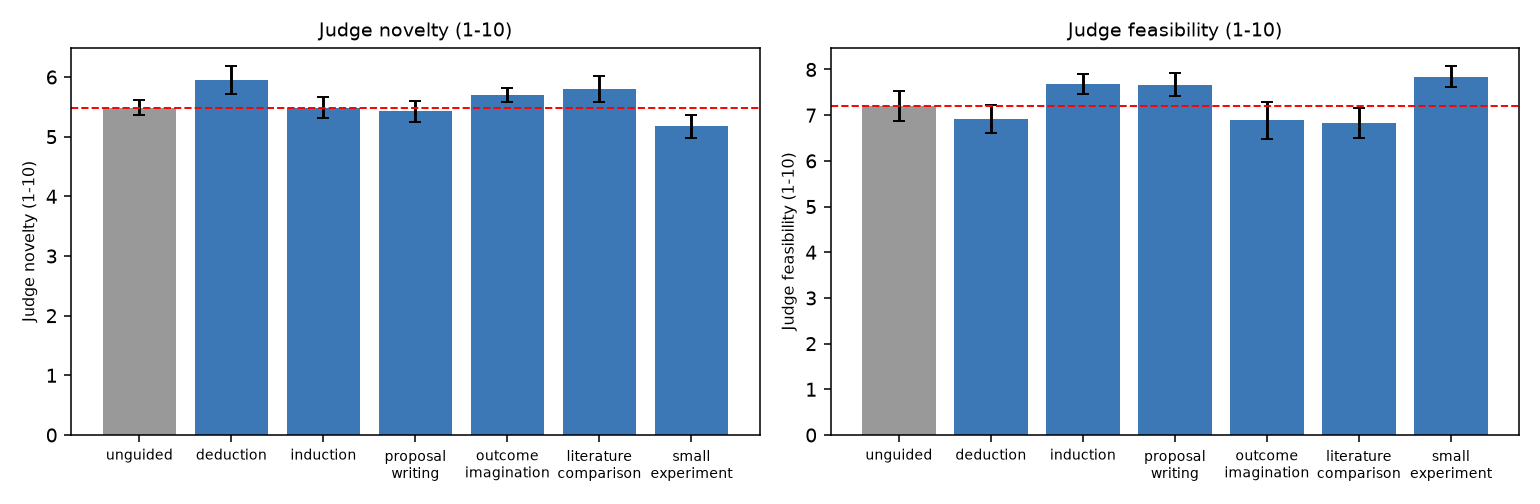
\includegraphics[width=\textwidth]{figures/fig2_judge_rubric.png}
        \caption{Rubric scores by condition}
        \label{fig:rubric}
    \end{subfigure}
    \hfill
    \begin{subfigure}[b]{0.48\textwidth}
        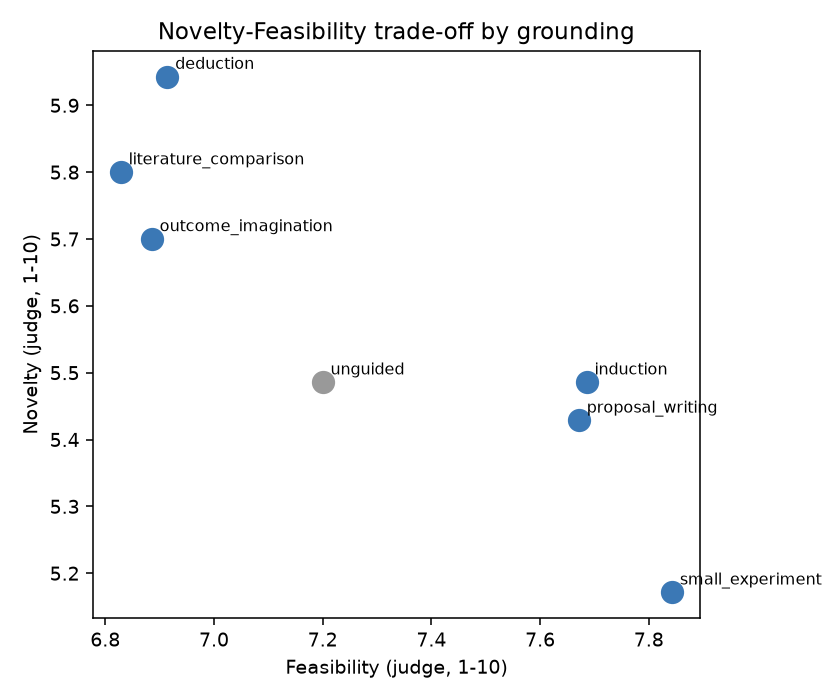
\includegraphics[width=\textwidth]{figures/fig3_tradeoff.png}
        \caption{Novelty--feasibility trade-off}
        \label{fig:tradeoff}
    \end{subfigure}
    \caption{Judge rubric results. \captiona Mean rubric scores by condition. \captionb Each condition placed on the novelty--feasibility plane relative to the control: generative grounding moves up-left (more novel, less feasible), validation grounding moves down-right (less novel, more feasible). Grounding is a steering knob, not a uniform quality lever.}
    \label{fig:judge}
\end{figure}

\para{Pairwise win-rate.} Pairwise judging is more sensitive than absolute scoring (\Tabref{tab:pairwise}, \Figref{fig:pairwise}). \litcomp is preferred over the control $79\%$ of the time ($p < 0.001$) even though its \emph{absolute} overall score was flat---a known absolute-versus-comparative judging gap. \outcome ($65\%$) and \deduction ($62\%$) also win significantly. At the other end, \smallexp is reliably \emph{dis-preferred} ($33\%$, $p = 0.005$), consistent with its low novelty and overall scores.

\begin{table}[t]
    \centering
    \caption{Pairwise win-rate $P(\text{grounded} \succ \unguided)$ on overall preference, position-controlled across 2 judges $\times$ 2 orderings ($n = 35$ per condition). \checkmark marks a significant win, {\footnotesize\textsf{X}} a significant loss, versus chance (0.5). Best in \textbf{bold}.}
    \label{tab:pairwise}
    \begin{tabular}{@{}lccc@{}}
        \toprule
        Condition & Win-rate & 95\% CI & $p$ vs.\ 0.5 \\
        \midrule
        \litcomp        & \textbf{0.79} & [0.71, 0.86] & $<0.001$~\checkmark \\
        \outcome        & 0.65 & [0.55, 0.74] & 0.006~\checkmark \\
        \deduction      & 0.62 & [0.51, 0.72] & 0.033~\checkmark \\
        \induction      & 0.46 & [0.37, 0.56] & 0.468 \\
        \proposal       & 0.43 & [0.33, 0.53] & 0.177 \\
        \smallexp       & 0.33 & [0.22, 0.44] & 0.005~{\footnotesize\textsf{X}} \\
        \bottomrule
    \end{tabular}
\end{table}

\begin{figure}[t]
    \centering
    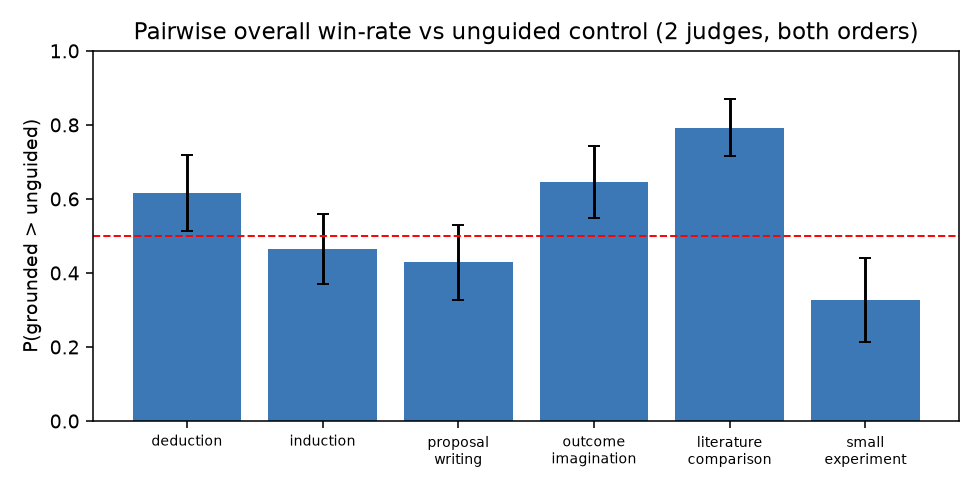
\includegraphics[width=0.62\linewidth]{figures/fig4_pairwise.png}
    \caption{Pairwise overall win-rate against the unguided control with bootstrap 95\% CIs; the dashed line marks chance (0.5). \litcomp wins $79\%$ of comparisons; \smallexp is reliably dis-preferred.}
    \label{fig:pairwise}
\end{figure}

\subsection{Set-level diversity}
\label{sec:res_div}

\Tabref{tab:diversity} reports within-cell diversity. Only \litcomp meaningfully increases mean pairwise distance ($0.456$ vs.\ $0.412$) while lowering the near-duplicate rate ($0.091$ vs.\ $0.106$), consistent with its retrieve-and-differentiate mechanism. The other conditions are at or slightly below the control. H4 is supported only for literature comparison; grounding does not broadly fix the diversity collapse documented by \citet{si2024can}. \Figref{fig:diversity} visualizes the ranking.

\begin{table}[t]
    \centering
    \caption{Set-level diversity within (condition $\times$ topic) cells. Higher mean pairwise distance and lower near-duplicate rate (cosine $\geq 0.8$) are better. Only \litcomp improves on the control for both. Best in \textbf{bold}.}
    \label{tab:diversity}
    \begin{tabular}{@{}lcc@{}}
        \toprule
        Condition & Mean pairwise dist.\ $\uparrow$ & Near-dup rate $\downarrow$ \\
        \midrule
        \litcomp        & \textbf{0.456} & \textbf{0.091} \\
        \smallexp       & 0.424 & 0.094 \\
        \unguided       & 0.412 & 0.106 \\
        \outcome        & 0.407 & 0.096 \\
        \deduction      & 0.404 & 0.104 \\
        \proposal       & 0.397 & 0.109 \\
        \induction      & 0.393 & 0.106 \\
        \bottomrule
    \end{tabular}
\end{table}

\begin{figure}[t]
    \centering
    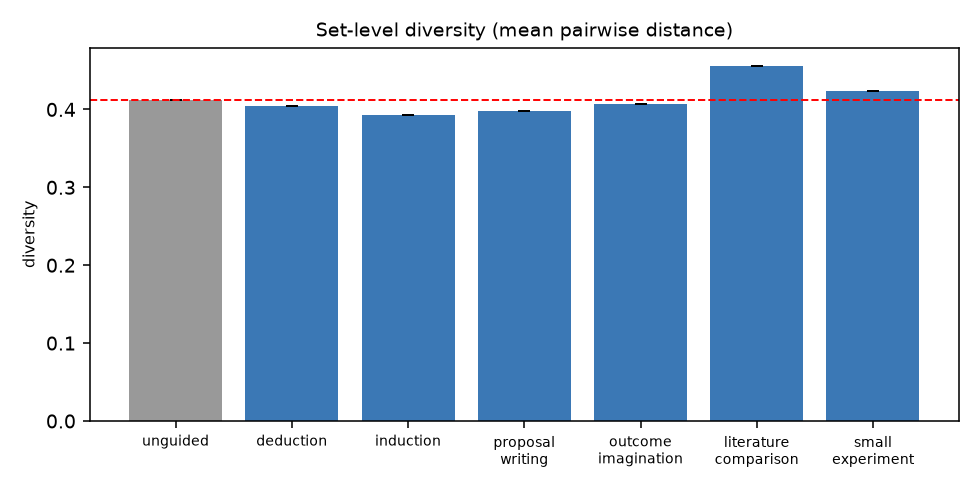
\includegraphics[width=0.6\linewidth]{figures/fig5_diversity.png}
    \caption{Mean within-cell pairwise distance by condition. Only \litcomp clearly exceeds the unguided control, matching its retrieve-and-differentiate design.}
    \label{fig:diversity}
\end{figure}

\subsection{Judge validation: the novelty mirage, measured}
\label{sec:res_valid}

The three lenses can only be reconciled by checking whether the judge measures what \lgn measures. It does not. The two judges \emph{agree with each other}: their novelty scores correlate at Spearman $\rho = 0.41$ ($p = 8 \times 10^{-11}$), moderate and significant, so the rubric is reliable enough to interpret. But judge novelty and objective \lgn are \emph{unrelated}: Spearman $\rho = 0.012$ ($p = 0.85$), essentially zero (\Figref{fig:convergent}). H5 is refuted. This is the crux: the judges reliably reward something, and that something is \emph{not} distance from prior work. The novelty gains in \secref{sec:res_judge} are real in the judges' shared eye and a mirage under a literature-anchored measure---a controlled, item-level reproduction of the novelty mirage~\citep{rqbench2026}.

\begin{figure}[t]
    \centering
    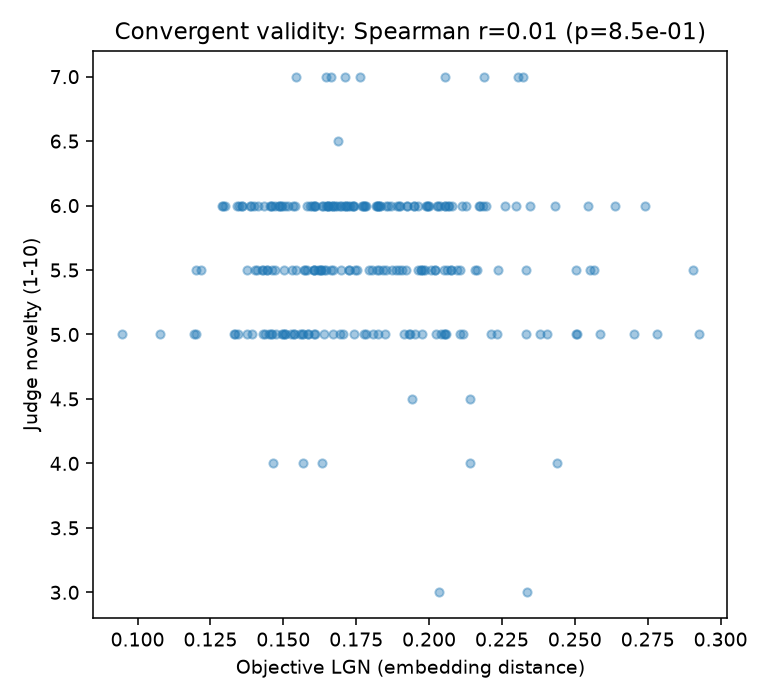
\includegraphics[width=0.6\linewidth]{figures/fig6_convergent.png}
    \caption{Convergent-validity scatter: mean judge novelty (1--10) versus objective \lgn at the item level. The flat trend (Spearman $\rho = 0.01$, $p = 0.85$) shows the two are uncorrelated, even though the two judges agree with each other ($\rho = 0.41$). LLM-judged novelty and literature-distance novelty are different constructs.}
    \label{fig:convergent}
\end{figure}

\section{Discussion}
\label{sec:discussion}

\para{Why grounding reshapes rather than improves.} A single qualitative case captures the mechanism. On the Factuality topic, from the same seed, the \smallexp scaffold produced ``Chain-of-Verification''---a real, already-published method---whereas \litcomp and \deduction produced more elaborated ``counterfactual chain-of-reasoning'' and ``counterfactual retrieval'' variants. Asking the model to predict whether a small test would pass optimizes for ideas that \emph{will} survive scrutiny, \ie safe, known techniques: lower novelty, higher feasibility. Asking it to flip an assumption or out-distance retrieved papers optimizes for differentiation: higher judged novelty, lower feasibility. Grounding is therefore best understood as a \emph{steering knob on the novelty--feasibility axis}, not a uniform quality lever. This reframes the survey ranking (graph-grounded $>$ Chain-of-Ideas $>$ vanilla): the apparent advantage of grounding may be a judged-novelty effect that our objective metric does not corroborate.

\para{The mirage is the most important result.} Judged novelty rises for \deduction and \litcomp, yet objective distance to prior work does not, and the two measures are uncorrelated at the item level ($\rho = 0.01$). Because the two off-family judges \emph{agree with each other} ($\rho = 0.41$), the mirage is not judge noise---they reliably reward something real, just not occupancy of unexplored regions of the literature. The reward goes to \emph{rhetorical} novelty: framing, elaborate mechanism descriptions, and signal words like ``counterfactual.'' This operationalizes the \emph{All That Glitters} warning~\citep{glitters2025} and reproduces RQ-Bench's mirage~\citep{rqbench2026} in a controlled setting where the idea set is held fixed and only the measurement changes. The practical consequence is direct: measure novelty as distance to retrieved prior work, not as an LLM's opinion, and never report a single-judge novelty number alone.

\para{Calibration against prior work.} Our control means (judge novelty $\approx 5.5$, feasibility $\approx 7.2$) sit in a plausible band relative to the human AI-condition means of \citet{si2024can} (novelty $\approx 5.6$, feasibility $\approx 6.3$), so the judges are not wildly miscalibrated in absolute terms---the problem is what they track, not their scale.

\para{Failure modes.} We observed three. (1)~\emph{Topic-anchored convergence}: ``counterfactual'' dominated the Factuality topic across conditions, with grounding modulating elaboration around the motif rather than escaping it. (2)~\emph{Rediscovery}: \smallexp repeatedly produced named existing methods. (3)~\emph{Scale compression}: the absolute rubric compresses ideas into the 5--6 band, hiding preferences that pairwise judging readily reveals (\eg \litcomp's flat absolute overall score but $79\%$ win-rate).

\para{Limitations.} (1)~\emph{Single backbone.} We fixed \gptfourone to isolate grounding, trading external validity for internal validity; mechanism effects may differ for other model families. (2)~\emph{No item-level human anchor.} The released Si review data is anonymized without idea text, so we could not correlate our judges against human scores item-by-item; we validated via inter-judge agreement and convergent validity instead, but the absent human anchor is a real gap. (3)~\emph{Thought-experiment grounding.} Generic ideas cannot be cheaply executed in-loop, so \smallexp is predict-and-critique rather than a real run; a domain where ideas \emph{are} runnable (\eg a fixed prompting benchmark) could test true experimental grounding. (4)~\emph{\lgn is one embedding model's view}; cosine distance to abstracts is a proxy, not ground truth---but it is judge-independent, so its disagreement with the judge is informative regardless of absolute calibration. (5)~\emph{Scale and scope.} $N = 5$ per cell gives medium power; under-powered trends (\eg \outcome novelty, $p = 0.09$) are suggestive only, and we tested single-mechanism scaffolds, not the 2--3-mechanism combinations most strong systems use. (6)~\emph{Contamination.} The public topics are within \gptfourone's training data, which may inflate the rediscovery failure mode.

\para{Broader implications.} Grounding is a cheap, deployable prompting protocol, and our results let practitioners pick the knob that matches their goal rather than chasing a single ``quality'' number. More broadly, the mirage result is a caution for the rapidly growing practice of using LLM judges to score machine-generated research: a metric that two strong judges agree on can still be measuring the wrong construct.

\section{Conclusion}
\label{sec:conclusion}

We ran the first controlled head-to-head ablation of six grounding mechanisms for LLM scientific idea generation, holding the backbone, topics, and output schema fixed and evaluating 245 ideas through an objective literature-distance metric, a 2-judge off-family rubric, and position-controlled pairwise comparisons. The answer to our research question is \emph{partial and conditional}: grounding does not uniformly produce better ideas; it \emph{steers} the novelty--feasibility trade-off. Deduction, literature comparison, and outcome imagination raise judged novelty and win pairwise against unguided generation---literature comparison most strongly ($79\%$), and it alone improves idea-set diversity---while small experiments, induction, and proposal writing raise feasibility at novelty's expense.

\para{Key takeaway.} No mechanism increases objective distance from prior work, and LLM-judged novelty is uncorrelated with that objective measure ($\rho = 0.01$) even though the two judges agree with each other. The hypothesized ``better novelty'' is real in human-style judgment but a mirage under a grounded metric. Concretely: for judged novelty, diversity, and head-to-head wins use literature comparison; for feasibility use induction or proposal writing; avoid small-experiment grounding when novelty matters, as it rediscovers known methods; and for evaluation, never report single-LLM-judge novelty alone---pair it with a literature-distance metric and pairwise comparison, because they can disagree completely.

\para{Future work.} Four directions follow. (1)~Replicate across backbones (Claude, Gemini, DeepSeek) to test generality. (2)~Combine mechanisms---\eg deduction followed by literature-comparison filtering---to seek novelty \emph{and} feasibility together. (3)~Build the missing item-level human anchor on fresh, post-cutoff ideas to calibrate which metric tracks expert judgment. (4)~Test true small-experiment grounding in a runnable prompting benchmark where ideas can be executed in-loop. We release our code, the 245 generated ideas, judge scores, and analysis to support these extensions.


\bibliography{references}

\end{document}
